% !TeX encoding = UTF-8
% !TeX root = ../main.tex
% !TeX spelling = en_GB
% !dsfaTeX program = latexmk

\chapter{Theory}
\label{chap:theory}

\subsection{Forming of Ice}

Apart from being a rather complex phenomenon in itself, icing on wind turbines is forming differently from the ice accretion on an aircraft airfoil. First since the turbine is stationary it cannot stop icing, or de-ice by moving to a different condition. Same conditions may also continue for days or weeks. Secondly the turbine blade moves concentrically making the tip of the blade the fastest, and occasionally highest moving part. The remote and exposed position of icing makes it difficult to detect ice directly when it is initially formed (Matthew C. Homola, Nicklasson, \& Sundsbø, 2006).

\subsection{Liquid Water Content and Median Volume Diameter}

The liquid water content (LWC) and the water droplets median volume diameter (MVD) are essential input parameters to predict or model icing. The  MVD is given at the point where half of the total volume of liquid content in a fixed air volume consists of droplets with diameters larger and the other half has smaller diameters. For estimation of icing, the MVD has been shown to be a good indicator (L. Makkonen, 1992).

Although there do exist methods to measure these properties, they are scarcely ever measured at a planned or existing wind turbine [9, 10]. Measuring them accurately and frequently would be an advantage for the planning of new wind mill farms or for the application of anti-icing arrangements on existing power stations. It may be of particular interest as input to weather prediction models by which both LWC and MVD can be computed [7, 8]. In combination with information about the aerodynamic properties of the wind turbine, it can give more accurate predictions of icing or even result in better design of wind turbines and anti-icing methods.

While icing caused by large supercooled droplets, with diameters from approximately 50 μm to exceeding 1000 μm, is often considered severe due to its shape and quick build-up, icing may occur even with droplets as small as 5 μm [11-13]. In most cases, though, icing is caused by cloud droplets measuring between 10 μm and 30 μm in diameter [10, 12].
Although optical imaging and other techniques for measuring aerosol properties is continuously improving, the choice of instrument is still very much dependent on the application’s requirements [14-17]. An instrument for measuring icing parameters for wind turbines should be able to detect supercooled cloud droplets from five micrometer and determine an accurate measure of the LWC. Since measurements are needed in multiple remote locations it should also be affordable, reliable, have low power consumption, and ideally be possible to place near the highest point of the turbine [18].


\section{Optical Properties}
Instruments based on Mie calculations of light scattering have the issue of dealing with aliasing in the sample bin resolution, leading to spikes in the size distribution (Evaluation of the Forward Scattering Spectrometer Probe-Baumgardner 1990, Spiegel Zieger 2012). 

\subsection{Light Spectrum}
 In visible light, water is almost transparent. This means that the imaginary part of the refractive index, i.e. the absorption, is very small, while for some higher and lower wavelengths it increases with a factor of almost ten power to ten (Segelstein, 2011). This fact is used in two-color lidar measurements (Westbrook, Hogan, O'Connor, \& Illingworth, 2010).

The real part of the refractive index for water is much more stable, approximately 1.34 at 455nm light (Hale \& Querry, 1973).

A spherical lens in the form of a droplet will scatter almost all of the light that reaches the droplet from different directions. Some of the light will also be absorbed, albeit the absorption of a single water droplet is negligible due to its small volume and because water absorb very little in the visible spectrum.

The combined effect of scattering and absorption is the extinction (Bohren \& Huffman, 2008). Due to this combined effect, clouds look nontransparent from a distance. Measuring extinction is possible in aerosols e.g. by using Raman LIDAR (Ansmann, Riebesell, \& Weitkamp, 1990).

\section{Materials}
\subsection{LED Light Source}

LEDs can sometimes be used with currents far above the specifications, as long as the pulse length is short and the duty cycle is low enough to permit the heat generated to be transported away between the pulses. Using the LED above specifications may though affect the efficiency and aging of the LED. LED emittance also depends on the temperature. Depending on the capacitance of the diode, the rise time may limit the current, although there exist some techniques to shorten the LED pulses (Tanaka, Umeda, \& Takyu, 2011; Veledar et al., 2007).

\section{Image Segmentation}

Edge detection can be done in several ways. The simplest method is to use a threshold at a fixed level and define the edge as the transition between above and below that threshold (Gonzales \& Woods, 2002). Other techniques use different methods to measure the gradient of the change in intensity (Canny, 1986; Marr \& Hildreth, 1980)


\section{The Impact}

Makkonen and rotating cylinders...

The icing process is complex and the result depends on a combination of the aerodynamic shape of the structure or airfoil, the velocity of the air and its contained water, the temperature, the mixing of snow and water, the concentration of liquid water and the droplet size distribution. The figure below illustrates the difference between large and small supercooled droplets passing an aerodynamic profile.

\begin{figure}%[h]
\centering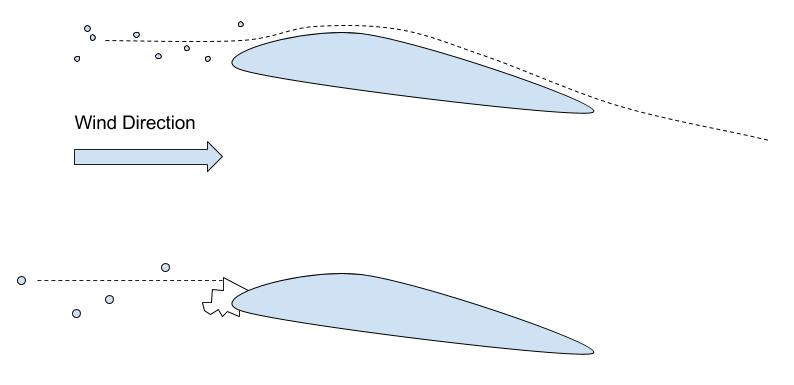
\includegraphics[width=0.6\linewidth]{figures/freezing_droplets}
\caption{Supercooled water droplets on collision course with an aerodynamic profile.}
\end{figure}


A particle’s eagerness to follow the flow or collide depends on several factors, like the flow velocity, the size of the obstacle, the density and drag coefficient of the particle. This relationship is known in fluid mechanics as the Stokes number (Stk). Small droplets or particles with Stk << 1 may continue with the airflow around the profile, while large droplets or particles with Stk >> 1 due to their inertia collide with the structure. A supercooled droplet colliding with a structure would likely freeze on the impact.

All droplets or particles approaching an obstacle are affected by the change in pressure and wind direction surrounding it, a fact which complicates measuring the concentration of particles in unaffected air. Measurement probes working by extraction of air using a mechanical air pump would expect a loss of particles with large Stokes numbers. Ideally the measuring device would affect the flow as little as possible.

Measuring particles from aircraft is complicated by the high air speed. The sample is affected by the change in pressure surrounding the aircraft and by particles hitting parts of the probe, splintering or changing direction. (ref) An instrument fixed to the ground on the other hand is affected by the wind speed relative to the ground. This means that it needs to be directed in the direction of the wind. Particles may also enter the measurement zone from different directions depending on their Stokes number, which has been shown to have a large impact on the measured liquid water content (ref).

